\documentclass{beamer}
\title{Nombre de la Unidad de Aprendizaje}
\date[today]{\today}
\author[Name]{CS1100 - Introducci\'on a Ciencia de la Computaci\'on}
\institute[Department]{UTEC}

\usetheme{lumc}
\usepackage{multicol} % 
%\usepackage{animate}  % animation
\usepackage{amsmath,amsfonts,amssymb} 
\usepackage{listings}
\lstset{basicstyle=\ttfamily,breaklines=true}

\newcommand{\estiloPython}{
\lstset{
    language=Python,
    basicstyle=\fontsize{15}{20}\ttfamily\ttfamily,
    keywordstyle=\color{jpurple}\bfseries,
    stringstyle=\color{red},
    commentstyle=\color{verde},
    morecomment=[s][\color{blue}]{/**}{*/},
    extendedchars=true,
    showspaces=false,
    showstringspaces=false,
    numbers=left,
    numberstyle=\normalsize,
    breaklines=true,
    backgroundcolor=\color{cyan!10},
    breakautoindent=true,
    captionpos=b,
    xleftmargin=0pt,
    tabsize=2
}}

\begin{document}

\begin{frame}
\titlepage
\end{frame}

%%%%%%%%%%%%%%%%%%%%%%%%%%%%%%%%%%%%%%%%%%%%%%%%%%
\section{Motivaci\'on}
%%%%%%%%%%%%%%%%%%%%%%%%%%%%%%%%%%%%%%%%%%%%%%%%%%
\begin{frame}[fragile]{Logro de la Sesi\'on} 
  \begin{block}{Al finalizar esta sesi\'on, estar\'as en la capacidad de:}
    \begin{itemize}[<+- | alert@+>]
      \item desarrollan programas en Python, utilizando funciones y recursividad.
    \end{itemize}
  \end{block}
\end{frame}

%%%%%%%%%%%%%%%%%%%%%%%%%%%%%%%%%%%%%%%%%%%%%%%%%%

\section{Adquisici\'on}

\begin{frame}[fragile]{Algoritmo recursivo}

{\Huge Es un algoritmo que expresa la soluci\'on de un problema en t\'erminos de una llamada a si mismo (llamada recursiva o recurrente}

\begin{figure}
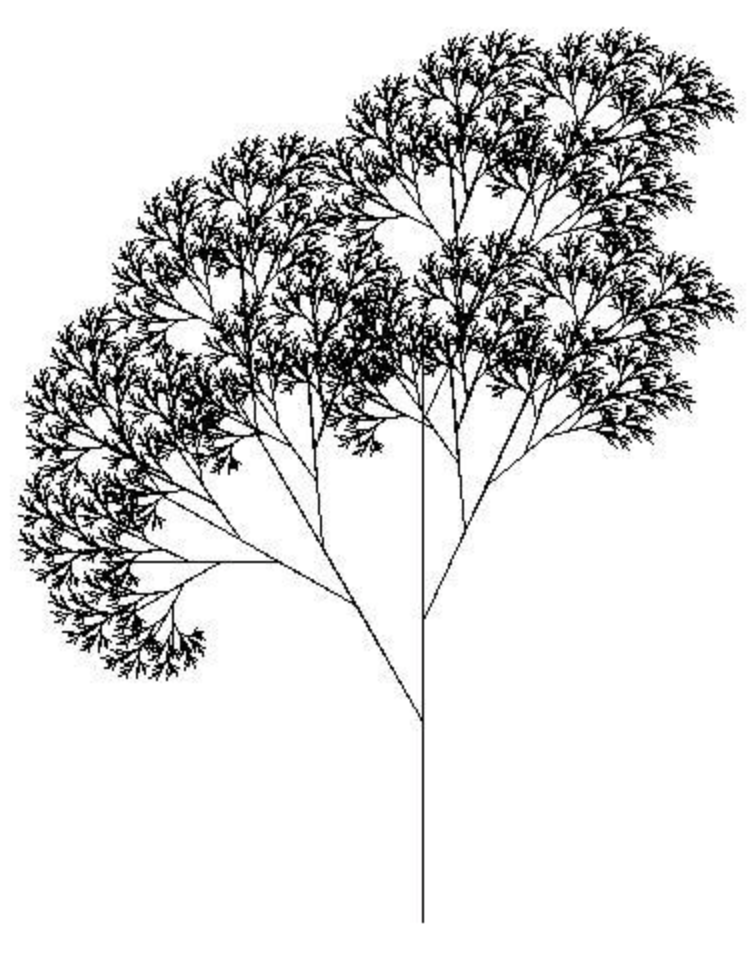
\includegraphics[width=0.4\linewidth]{08.png}
\end{figure}
\end{frame}

%%%%%%%%%%%%%%%%%%%%%%%%%%%%%%%%%%%%%%%%%%%%%%%%%%
\section{Transferencia}
%%%%%%%%%%%%%%%%%%%%%%%%%%%%%%%%%%%%%%%%%%%%%%%%%%
\begin{frame}[fragile]{Algoritmo recursivo: Inverso de una cadena}

{\Large Sea una cadena obtener la cadena invertida
\begin{equation}
  suma(a,b)=\begin{cases}
    si \ s=" " \ retornar " "\\
    Retornar \ inverso(s[1:]) + s[0]
  \end{cases}
\end{equation}
}
\begin{figure}
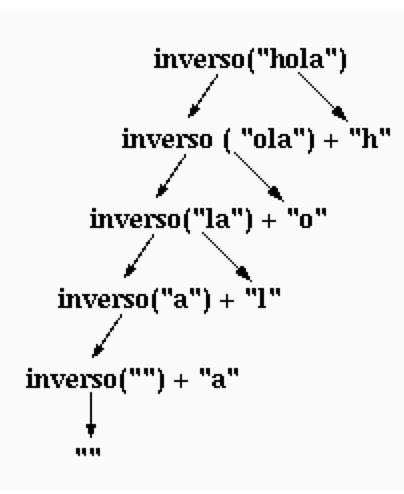
\includegraphics[width=0.2\linewidth]{06.png}
\end{figure}
  \estiloPython
\begin{lstlisting}[frame = single]
""" inverso de una cadena"""
def inverso(s):
if s == ' ':
return ' '
else:
return inverso(s[1:]) + s[0]
print(inverso('hola como estas'))
\end{lstlisting}
\end{frame}

%%%%%%%%%%%%%%%%%%%%%%%%%%%%%%%%%%%%%%%%%%%%%%%%%%
\begin{frame}[fragile]{Generar la secuencia de Fibonacci para el n�mero N}
\begin{figure}
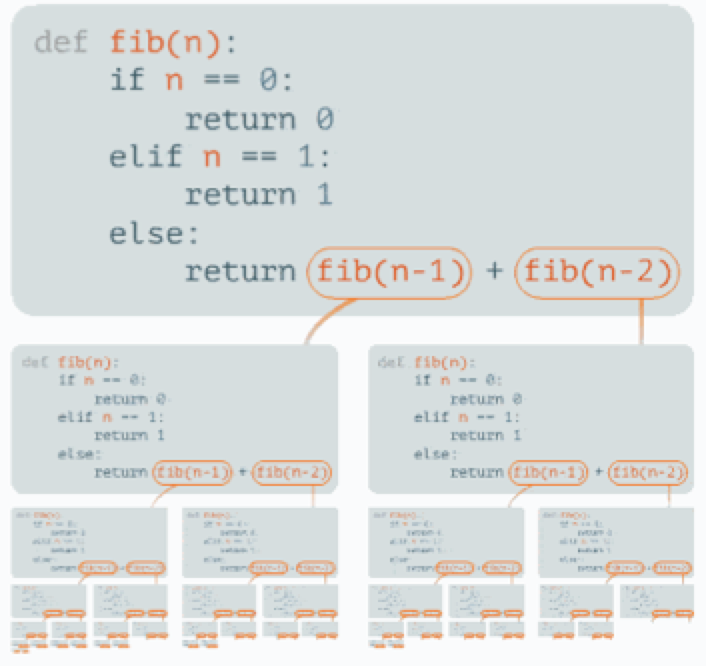
\includegraphics[width=0.5\linewidth]{07.png}
\end{figure}
\end{frame}

%%%%%%%%%%%%%%%%%%%%%%%%%%%%%%%%%%%%%%%%%%%%%%%%%%
\section{Evaluaci\'on o Cierre}
%%%%%%%%%%%%%%%%%%%%%%%%%%%%%%%%%%%%%%%%%%%%%%%%%%
\begin{frame}[fragile]{Ejercicio 1}
  \begin{block}{Enunciado}
Escribir una funci\'on recursiva que calcule la multiplicaci\'on de un n\'umero por 5
    \end{block}

\end{frame} 

%%%%%%%%%%%%%%%%%%%%%%%%%%%%%%%%%%%%%%%%%%%%%%%%%%

\begin{frame}[fragile]{Ejercicio 2}
  \begin{block}{Enunciado}
?`Cu\'al ser\'a el capital de 10K Soles despues de 10 a\~nos si el inter\'es anual es del 8\%? Programe la soluci\'on con una funci\'on recursiva
   \end{block}
\end{frame} 

%%%%%%%%%%%%%%%%%%%%%%%%%%%%%%%%%%%%%%%%%%%%%%%%%%
\begin{frame}[fragile]{Ejercicio 3}
  \begin{block}{Enunciado}
La cantidad de bacterias en un cultivo se triplica cada hora. ?`Cu\'antas bacterias habr\'an despues de 10 horas? Programe la soluci\'on con una funci\'on recursiva
   \end{block}
\end{frame} 

%%%%%%%%%%%%%%%%%%%%%%%%%%%%%%%%%%%%%%%%%%%%%%%%%%


\begin{frame}[fragile]{Evaluaci\'on}
  \begin{exampleblock}{Individual Work}
  \begin{itemize}
  \item \href{www.hackerrank.com/cs1100-lab-01
}{www.hackerrank.com/cs1100-lab-01}
  \end{itemize}
\end{exampleblock}    
\end{frame} 

%%%%%%%%%%%%%%%%%%%%%%%%%%%%%%%%%%%%%%%%%%%%%%%%%%

\begin{frame}[fragile]{Cierre} 
  \begin{block}{En esta sesi\'on aprendiste:}
    \begin{itemize}[<+- | alert@+>]
      \item desarrollan programas en Python, utilizando funciones y recursividad.
    \end{itemize}
  \end{block}
\end{frame}


\end{document}